\documentclass[letterpaper]{article}

\usepackage{amsmath, hyperref, enumerate, comment}
\usepackage{amsfonts, esint}
\usepackage{graphicx}
\usepackage{mathrsfs} %for script font 

\usepackage[backend=biber, style=authoryear, url=false, doi=false, eprint=false]{biblatex}
%\usepackage[backend=biber,  style=authoryear-icomp, url=false, doi=false, eprint=false]{biblatex}
\addbibresource{bibliography.bib}

\AtEveryBibitem{%
  \clearfield{note}%
  \clearfield{series}%
  \clearfield{pages}%
}


\newcommand{\diff}{\mathop{}\!\mathrm{d}} %defines exterior derivative 
\renewcommand{\div}[1]{\gv{\nabla} \cdot #1} % for divergence
\newcommand{\curl}[1]{\gv{\nabla} \times #1} % for curl
\renewcommand{\vector}[1]{\ensuremath{\vec{#1}}} % redefines vector to vec
\newcommand{\integral}{\int}


\begin{document}
%% testing from desktop

\title{TBD}
\author{TBD}

\date{\today}

\maketitle

\begin{abstract}
	TBD
\end{abstract}


Current section ideas:

\begin{enumerate}[1.)]

\item Assumptions of physics framework section

\begin{itemize}

\item motivate everything upfront: going to show that Hamiltonian mechanics corresponds to two conditions being satisfied, while Lagrangian mechanics requires a third condition
\item define the two assumptions, and give motivation
\item figuring out which mathematical structures are required for systems that satisfy certain physical conditions
\item go over the upshot of the philosophical argument, specifically how this avoids the worries about measuring the amount of structure that plagued North (i.e. Swanson and Halvorson paper)
\item Then, give the derivation, as gentle and well-motivated as possible. But would be ideal if readers could skip or skim this section and still get the philosophical upshot, relatively early on.

\end{itemize}

\item Physical significance of invariant distributions

\begin{itemize}

\item explain how these provide a novel way of understanding things, one that we can physically privilege

\item connect this with North on invariant structure, but disavow metaphysical commitments


\end{itemize}

\item How to interpret Lagrangian mechanics in light of Hamiltonian mechanics

\begin{itemize}

\item gauge transformation stuff
\item go over the cool stationary action principle derivation/argument
\item clarify the status of Riemannian metric structure in the Lagrangian formalism
\item respond to Curiel's privileging of Lagrangian mechanics
\item respond to Curiel's argument that Hamiltonian mechanics involves the imposition of an ad hoc condition in order to get the right kinematical constraints, whereas these fall out naturally from Lagrangian mechanics.


\end{itemize}

\item Considerations in light of categorical equivalence proofs

\begin{itemize}

\item  clarify that argument is not in tension with categorical equivalence within the hyper regular domain. make this precise.
\item Respond to the worry that something must have gone amiss if we have a difference in the number of conditions required for the Hamiltonian vs. Lagrangian mechanics, yet still have categorical equivalence in the hyper-regular domain

\end{itemize}

\end{enumerate}

\section{Introduction}


% TODO: Lagrangian assumption vs kinematic assumption. Investigate what happens when the transformation is non-linear.

Philosophers have recently shown that we can interpret Lagrangian and Hamiltonian mechanics as theoretically equivalent in a precise mathematical sense. Within a subclass of classical mechanical systems known as the \textit{hyper-regular domain}, the two formalisms are categorically equivalent \parencites[]{Teh}{Barrett2}. Categorical equivalence provides a natural interpretive criterion for theoretical equivalence because it yields mutual inter-translatability between theory formulations. At first glance, this equivalence seems to motivate the view that there are no physically significant differences between these two formalisms, at least within the hyper-regular domain. This equivalence undermines prior positions that have privileged either Hamiltonian mechanics or Lagrangian mechanics on physical or metaphysical grounds \parencites[]{North}{Curiel}. Here, we will argue that there are indeed physical grounds for privileging Hamiltonian mechanics over Lagrangian mechanics, their categorical equivalence notwithstanding. Compared to Hamiltonian systems, an additional physical condition must be satisfied for a classical system to be Lagrangian. Hamiltonian mechanics thereby captures a wider range of systems than Lagrangian mechanics, and this difference has interpretive consequences even within the hyper-regular domain. Furthermore, the construction at the heart of this argument provides an interpretation of classical mechanical systems in terms of their invariant phase space density, along with a novel interpretation of the principle of stationary action within the Hamiltonian formalism.

Thesis: despite the mathematical equivalence of Hamiltonian and Lagrangian mechanics within the hyper-regular domain, the two frameworks have important differences. In particular, Hamiltonian systems arise when a smaller number of basic physical conditions are met. A Lagrangian system must satisfy a further physical condition. This shows that Hamiltonian mechanics is in a sense more fundamental. Defending this claim does not require commitments to fundamental structure or perfectly natural properties. (Furthermore, the Hamiltonian framework is more general because a Hamiltonian defines a unique solution (unique evolution in phase space) even when the Hessian is zero. In contrast, whenever the Lagrangian is not hyper-regular, the Euler--Lagrange equations do not possess a unique solution. Additionally, density plays a special role in the Hamiltonian framework, whereas it is in some sense an accident that the density in configuration space is invariant (simply because the Jacobian equals unity in Cartesian coordinates).

%Note that the photon does not belong to the hyper-regular domain. Furthermore, if you are not in the hyper-regular domain, then there is no longer a one-to-one map between position and velocity. 

Targets: Curiel's privileging of Lagrangian mechanics and argument that Hamiltonian mechanics is ad hoc; North's somewhat flawed privileging of Hamiltonian mechanics on the basis of it requiring less structure; a motivation stemming from categorical equivalence proofs for thinking that there are no physically significant differences between the Hamiltonian and Lagrangian frameworks (at least within the hyper regular domain).

Goals: provide a gentle introduction to Assumptions of Physics framework, and show that it has real philosophical payoffs for interpreting physical theories, such as classical mechanics.

\section{Defining `classical mechanical systems'}

Provide any relevant background on classical mechanics, specifically to clarify/define terminology. Might be able to just put this in the introduction proper, or the start of the next section. Make explicit how our terminology relates to other standard terminology in the philosophical literature.

A classical Hamiltonian system is any system whose phase space is a symplectic manifold and that evolves according to Hamiltonian evolution (i.e. according to a symplectomorphism). 

Throughout, we will focus only on non-dissipative classical systems, i.e. conservative systems. For in the context of transforming between the Hamiltonian and Lagrangian formulations (via a Legendre transform), we assume that the conjugate momentum $p$ is the derivative of the Lagrangian with respect to the generalized velocity $v $. This requires that the system is conservative, which is equivalent to the system being deterministic and reversible. Consequently, we will not consider systems that satisfy inhomogenous Euler--Lagrange equations.
% Dissipative systems contain more information than contained in the Lagrangian alone, namely, the additional information contained in the Rayleigh potential

\section{Privileging Hamiltonian mechanics}

Our framework develops a correspondence between three physical conditions and their associated mathematical formalisms. In this way, we straightforwardly interpret the physical significance of these mathematical formalisms. First, a system is \textit{infinitesimally reducible} provided that the states of its constituent, infinitesimal particles completely specify the overall state of the system. When this condition is satisfied, we can define a distribution $\rho$ over particle states. Furthermore, since particle states are independent of a choice of units, this distribution must be invariant. We show in Section~\ref{infinitesimal} that any infinitesimally reducible system has a phase space given by a symplectic manifold. The physical significance of this symplectic manifold is thereby its connection with the physical condition of infinitesimal reducibility. 

Secondly, a system has \textit{deterministic and reversible evolution} provided that the present state of the system uniquely determines both its future and past states. This condition entails that the preceding invariant distribution is in fact a conserved phase space density. We can thus model such systems using Hamiltonian mechanics, defined on a phase space with a symplectomorphism. These two conditions thereby characterize Hamiltonian mechanics as the mathematical framework for infinitesimally reducible systems with deterministic and reversible evolution. Section~\ref{deterministic} provides this derivation in detail.

Finally, a system satisfies a further condition---motion equivalence---when its trajectory in physical space determines and is determined by its evolution in phase space. This condition leads to a correspondence between velocity and momentum, which formally leads to the framework of Lagrangian mechanics in the hyper-regular domain (Section~\ref{motion}). Hence, Lagrangian mechanics requires that a further physical condition is satisfied, and hence it is less general than Hamiltonian mechanics. To see this, note that some systems fail to satisfy the condition of motion equivalence, i.e. it is not always true that we can determine the evolution of a system in phase space from its trajectory in physical space. For instance, knowledge of the trajectory of a photon is insufficient for knowledge of its phase space evolution, since we cannot determine the momentum of a photon from its trajectory alone. In general, different Lagrangians---differing even by more than a constant---can correspond to the same particle trajectories while not agreeing on the total energy, even up to a constant.\footnote{\textcites[1185--1186]{Barrett2} discusses this in the context of the failure of equivalence between the vector field formulations of Lagrangian and Hamiltonian mechanics. In contrast, the trajectories in phase space (encoded by the Hamiltonian vector field) uniquely define the Hamiltonian up to a constant.} Hence, the set of classical systems that satisfy this further physical condition is a proper subset of the classical systems that satisfy the conditions for Hamiltonian mechanics. On these grounds, we will argue in Section~\ref{fundamentality} that Hamiltonian mechanics is more fundamental than Lagrangian mechanics.
[To do: verify that the scenario of two different Lagrangians giving rise to the same trajectories in physical space with different energies, arises only when motion equivalence condition fails. See Curiel 2014, page 42 for his take on this kind of scenario.]

% One way to motivate the motion equivalence condition: in general, the same trajectory in physical space can correspond to different trajectories in phase space: knowledge of the position and velocity is not sufficient for knowledge of the momentum (e.g. if you do not know the mass of the system). Formally, different Lagrangians can have the same Lagrangian vector field but give rise to Hamiltonians with different Hamiltonian vector fields, as Barrett notes \parencites*[1186]{Barrett2}. In contrast, if two Hamiltonian systems agree on the Hamiltonian vector field, then they must agree on the Hamiltonian, up to an arbitrary constant (whereas two Lagrangian systems can have the same Lagrangian vector field but not agree on the Lagrangian or total energy, even up to a constant)).

% Overall summary: A classical system is an infinitesimally reducible system. The state space of these systems can be modeled by a symplectic manifold (the physical assumption of infinitesimal reducibility corresponds to the mathematical structure of symplectic manifolds). Classical Hamiltonian systems satisfy the additional conditions of having deterministic and reversible evolutions. These two physical assumptions entail the existence of a symplectic morphism on the state space manifold, making it a contact manifold. Classical Lagrangian systems satisfy a further assumption: keeping track of the trajectories in physical space is equivalent to tracking the evolution of states in phase space. 

Figure~\ref{diagram} summarizes our characterization of Hamiltonian and Lagrangian mechanics, in terms of physical conditions and corresponding mathematical structures. The left column lists the three physical conditions: infinitesimal reducibility, determinism/reversibility, and motion equivalence. Each condition entails physically significant properties, described in the middle column. Each of these physical properties corresponds to a formal mathematical framework, described in the right column. Section~\ref{derivation} justifies the logical connection between these physical conditions and corresponding mathematics. Before delving into this derivation, Section~\ref{fundamentality} discusses its philosophical significance.

\begin{figure}[h]
	\centering
	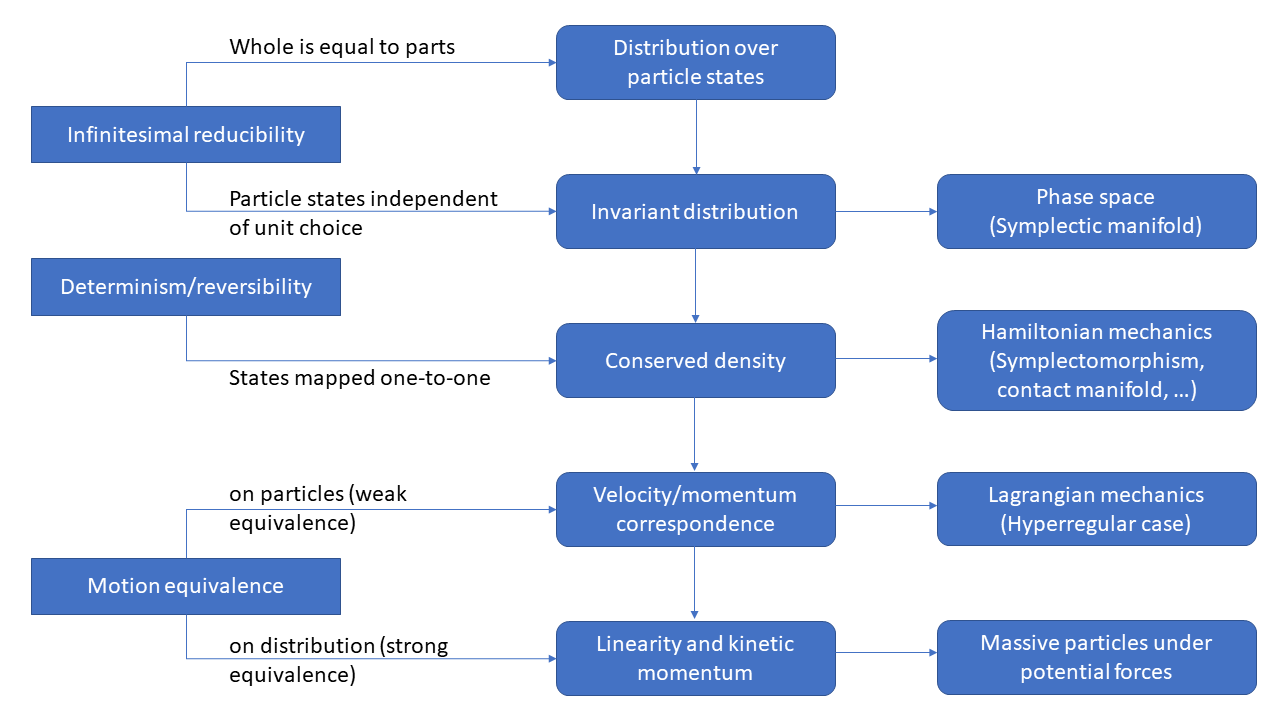
\includegraphics[width=\textwidth]{Diagram.png}
\caption{Physical conditions and corresponding properties and formalisms}
\label{diagram}
\end{figure}

\subsection{Fundamentality and structure}
\label{fundamentality}


In claiming that Hamiltonian mechanics is more fundamental than Lagrangian mechanics, we must clarify what we mean by ``fundamental." Of the various notions of fundamentality, there is at least the following non-mysterious definition: a formalism is more fundamental provided that it is logically more general. In this case, the Lagrangian framework is less general because it requires that an additional condition hold, compared to the Hamiltonian framework. Hence, the Lagrangian framework is less fundamental because it is a proper subset of the Hamiltonian framework. In particular, the assumption of motion equivalence places an additional constraint on the Hamiltonian, a constraint that need not be satisfied in general. This notion of fundamentality leads as well to a concomitant notion of ``structure." Hamiltonian mechanics employs less structure than Lagrangian mechanics because the former requires that fewer physical conditions are satisfied. In Section~\ref{distribution}, we will discuss another sense in which the Hamiltonian formalism is more fundamental than Lagrangian mechanics.
% Way to motivate that the motion equivalence assumption further constrains the Hamiltonian: the Hamiltonian already defines a relationship between conjugate momentum and velocity (through ($dq/dt = \partial H / \partial p$) ). Motion equivalence provides a further constraint on this relationship, and hence a further constraint on the Hamiltonian. \\

% As defined, our notions of fundamentality and structure are not metaphysical in nature.

[Explain how our notion of comparative structure avoids the objections of Halvorson/Swanson against North's comparative notion of amount of structure.] \\

We do not endorse a metaphysical notion of fundamentality, on which a formalism is more fundamental provided that it is more joint-carving. For instance, North provides the following definition of structure: ``structure comprises the objective, fundamental, intrinsic features, the ones that remain the same regardless of arbitrary or conventional choices and description" \parencites*[66]{North}. While Hamiltonian mechanics is significant partly because it elucidates invariant distributions (Section~\ref{distribution}), we will also argue that classical mechanics deploys physically significant representations that are not intrinsic to mechanical systems. Additionally, whereas North \parencites*[76]{North} seeks to determine the ``real" fundamental state space structure of the theory---and correspondingly, of a classical world---we remain neutral on this underlying metaphysical question. Whether Hamiltonian phase space structure is metaphysically fundamental does not matter for the questions we seek to answer. Regardless of its metaphysical status, Hamiltonian mechanics is epistemically, conceptually, and physically more fundamental.

% Part of the following paragraph seems redundant given the preceding. Think about how to combine.
Methodologically, we agree with North that it is important to identify invariants and more generally ``the mathematical structure needed to formulate the theory in an invariant, frame-independent way" \parencites*[65]{North}. Additionally, we agree that it is worthwhile to identify what particular mathematical structure is required by a formulation \parencites[78]{North}. However, whereas North proceeds mainly from the mathematical structure to claims about physical significance, we seek to interpret the mathematics by beginning with physically significant assumptions. We seek to determine which physical assumptions are necessary and sufficient for supporting a corresponding mathematical structure. This does not entail that additional mathematical structure is necessarily physically insignificant or surplus structure, just that it may correspond to an additional physically significant assumption that might apply to the system under consideration. As we will see, this characterizes the relationship between Hamiltonian and Lagrangian formalizations of a classical system. Hence, whereas North views the Lagrangian structure as surplus or redundant (``excess, superfluous structure"), we take the Lagrangian structure as unnecessary but still physically significant, corresponding to an additional physical assumption that applies to some classical systems.

Furthermore, our argument does not privilege any one of the at least three different mathematical ways of formalizing Hamiltonian mechanics [mention these three formalisms and provide references]. Each of these frameworks has different pragmatic costs and benefits. Hence, unlike North, we are comfortable acknowledging that the mathematical structure that you ``need" might not be unique. There might not be a single canonical minimal structure for formalizing the relevant physical models and physical assumptions. Neither one of these three formalizations of Hamiltonian mechanics is necessarily more ``fundamental" or joint-carving than the others. And in some sense, each of these formalisms references some ``unphysical" coordinates or representational means. Nevertheless, there are compelling physical and pragmatic motivations for preferring the extended phase space formulation of Hamiltonian mechanics. In this formulation, we gain an invariant Hamiltonian that is the conjugate variable of the proper time, while the normal Hamiltonian (which is not coordinate-invariant) still plays the role of generating time-translations.
% One con of this extended phase space formulation: the Hamiltonian constraint is both a constraint and the generator of time evolution; hence, it must be defined in the neighborhood of the actual states, so the values it provides outside of these neighborhoods should be unphysical, yet they encode the equations of motion.
% Should we remark on the claim that the only structure we need is whatever is sufficient to define densities locally? Hence, we need just the symplectic form but not the cotangent bundle?
% E.g. in the extended phase space formulation, the equations of motion come from derivatives of the Hamiltonian constraint over the variables, but this constraint is defined on unphysical points. These unphysical points are plausibly a mathematical artifact, although they supply a nice tool/method for understanding physically significant aspects of the representation.

% One way to motivate the motion equivalence condition: in general, the same trajectory in physical space can correspond to different trajectories in phase space: knowledge of the position and velocity is not sufficient for knowledge of the momentum (e.g. if you do not know the mass of the system). Formally, different Lagrangians can have the same Lagrangian vector field but give rise to Hamiltonians with different Hamiltonian vector fields, as Barrett notes \parencites*[1186]{Barrett2}. In contrast, if two Hamiltonian systems agree on the Hamiltonian vector field, then they must agree on the Hamiltonian, up to an arbitrary constant (whereas two Lagrangian systems can have the same Lagrangian vector field but not agree on the Lagrangian or total energy, even up to a constant)).


Claim to think about: GC was arguing on 10-12 that you could handle classical systems in the Hamiltonian framework with just a differential manifold and no symplectic structure. This would contradict North's indispensability claim that Hamiltonian symplectic structure is necessary for treating classical systems. E.g., North footnote 31: ``The symplectic form is crucial to determining the motion, since the same Hamiltonian can induce different flows for different symplectic forms" [76]. North takes this as an argument for why we cannot eliminate the symplectic form in an attempt to get at even less structure. We need it to define the dynamics.

% North argues that ``the structure of physics is the (minimal) structure that is assumed among dynamically equivalent---in classical mechanics: canonically transformed---formulations of a theory. Structure comprises those quantities that remain intact when we transform one allowable coordinatization of the laws into another" [78]

% North definition of structure: ``structure comprises the objective, fundamental, intrinsic features, the ones that remain the same regardless of arbitrary or conventional choices and description" [66]. So presumably, North would view the invariant phase space density as part of this fundamental structure.

% North's epistemic method for figuring out the structure: ``look at what is invariant under allowable transformations"; this tells us what the structure is [73].

\section{Derivation}
\label{derivation}

Sections~\ref{infinitesimal}-\ref{deterministic} show how to derive the formalism of Hamiltonian mechanics from the assumptions of infinitesimal reducibility and deterministic/reversible evolution. Section~\ref{motion} shows how systems that satisfy the further condition of motion equivalence can be treated within the formalism of Lagrangian mechanics.

\subsection{Infinitesimal reducibility}
\label{infinitesimal}

First, we will show that a classical phase space arises if and only if a system satisfies the following physical condition:

\begin{quotation}
\noindent
\textit{Infinitesimal reducibility}: the state of the system is reducible to the state of its infinitesimal parts. That is, giving the state of the whole system is equivalent to giving the state of its parts, which is equivalent to giving the states of those parts, and so on.
\end{quotation}

\noindent
This assumption characterizes classical systems as those whose infinitesimal parts completely specify the state of the system. [At least in a footnote: comment on how this characterization of infinitesimal particles relates to standard philosophy of physics interpretive disputes over the status of point particles in classical mechanics. See Butterfield Pointillisme article; Butterfield characterizes particles as extensionless.]

Let $\mathcal{C}$ be the state space for the whole system. Any point $c \in \mathcal{C}$ represents a particular state of the whole system. We define a classical \textit{particle} as the limit of recursive subdivision. A classical system then consists of a collection of classical particles. Let $\mathcal{S}$ be the state space for the particles, so that each point in $\mathcal{S}$ describes a possible state of a classical particle. We assume that this state space $\mathcal{S}$ is a manifold. Then for each state $c \in \mathcal{C}$ there exists a unique distribution $\rho_c : \mathcal{S} \to \mathbb{R} $ that describes the state of $c$'s parts. That is, the state of the whole system is a distribution over its infinitesimal parts. This distribution describes the proportion of classical particles in any particular state. Formally, if $\mathcal{S}$ is a manifold, $\int_U \rho_c d\mathcal{S}$ gives us the fraction of the system whose parts are in the region $U$ of the state space $\mathcal{S}$. 
%[is region U in the state space C or S. I assume in S.].

We define the \textit{state variables} as a set of quantities $\xi^a$ that fully identify a state. Formally, $\xi^a: \mathcal{S} \to \mathbb{R}^n$, yielding a real-valued vector for any given particle state, with $n$-many degrees of freedom.\footnote{In the language of manifolds, these $\xi^a$ are called `coordinates,' but we will reserve that terminology for the state variables that define units.} We will define a \textit{coordinate} $q \in \xi^a$ as a particular state variable that defines a unit.  For instance, $q$ might be position, defining units of meters. In general, the coordinates are the subset of the state variables that define the unit system, needed to measure properties of the system. 

On physical grounds, the distribution $\rho_c$ must transform as both a density and a scalar function. As a function defined over the state variables, the distribution transforms as a density, i.e. $\rho_c$ changes as a function of the Jacobian determinant that relates the new coordinates to the old coordinates. As a function defined over the points in phase space, the distribution transforms as a scalar, i.e. $\rho_c$ is invariant under all coordinate transformations. Hence, the Jacobian determinant must in fact equal one. In other words, $\rho_c$ is a function only of the point $c$ and does not depend on the choice of coordinates.\footnote{Formally, we can express this argument as a chain of equalities: $\rho_c(\hat{\xi}^b)=\rho_c(s(\hat{\xi}^b))=\rho_c(s(\xi^a))=\rho_c(\xi^a) = \left|\frac{\partial \hat{\xi}^b}{\partial \xi^a} \right| \rho_c(\hat\xi^b)$, where $\rho_c(\hat{\xi}^b)$ is the distribution defined over the transformed state variables, and $\rho_c(s(\hat{\xi}^b))$ is the distribution defined over the points of phase space, where $s: \mathbb{R}^n \to \mathcal{S}$ an invertible function  mapping a particular value of the units $\hat{\xi}^b$ to a point in the particle phase space $\mathcal{S}$.} We will now show that in order for the distribution to satisfy these two constraints, the classical phase space must be at least a symplectic manifold. In other words, having symplectic manifold structure is a necessary condition for the distribution over particle states to transform as a density and scalar function.
%This is because the distribution is a function only of the states, rather than of the particular choice of coordinates. 
 % Classical phase space (i.e. a symplectic manifold) is the only space that satisfies these constraints on the distribution. 
%(in manifold terminology, these are known as coordinates)

The argument begins with the simplest case: suppose that a single coordinate $q $ suffices to define the unit system for the particle state space. Then, the state variables are given by a set $\xi^a = \{ q, k^i \}$, where \textit{prima facie} the index $i$ can range over more than one number. We will show that, in fact, there can only be a single $k^i$ variable in this case, conjugate to the single $q$ coordinate. Assuming that the particle density $\rho_c$ is a scalar, it follows that we can arbitrarily change the unit defined by $q$ without changing the density $\rho_c$. 
% We further assume that $q$ fully defines the units for all state variables. [Is there a way to physically motivate this assumption, beyond this being a constitutive role of the position-like state variables?]

Now, suppose that we change the units by transforming the coordinate $q$ to a new coordinate $\hat{q}$. Since---by assumption---$q$ fully defines the unit system, $\hat{q}$ must do so as well, making it a function just of the old coordinate: $\hat{q}=\hat{q}(q)$. Call the new units $\hat{\xi}^b = \{ \hat{q}, \hat{k}^i\}$. As shown above, the Jacobian determinant $\left|\frac{\partial \hat{\xi}^b}{\partial \xi^a} \right|$ must equal one. Assume for contradiction that there is only one state variable, so that there are no $k^i$ variables. Then we would have $\left|\frac{\partial \hat{\xi}^b}{\partial \xi^a} \right| = \left|\frac{\partial \hat q}{\partial q} \right| = 1$. But this would mean the unit change cannot be arbitrary. Therefore we must have two or more state variables, so that there must be at least one $k^i$ variable. 

\begin{comment}
%Longer justification for the Jacobian determinant equaling one. 

 As defined, $\rho_c$ is a function from the particle state space $\mathcal{S}$ to the reals. We can define $\rho_c$ on the units by taking advantage of an invertible function $s: \mathbb{R}^n \to \mathcal{S}$ mapping a particular value of the units $\hat{\xi}^b$ to a point in the particle phase space $\mathcal{S}$. Hence, by definition $\rho_c(\hat{\xi}^b):= \rho_c(s(\hat{\xi}^b))$. [Is this function $s$ the inverse of the coordinate mapping $\xi^b$?]. Then, since the physical state is independent of the coordinates, the state $s(\hat{\xi}^b)$ is the same state as $s(\xi^a) $ defined in terms of the original units $\xi^a$. Again, by definition, $\rho_c(s(\xi^a))=\rho_c(\xi^a) $. Since the distribution transforms as a density, it follows that $\rho_c(\xi^a)$ must equal the product of the Jacobian determinant $\left|\frac{\partial \hat{\xi}^b}{\partial \xi^a} \right| $ times the density defined over the transformed units: $\rho_c(\xi^a) = \left|\frac{\partial \hat{\xi}^b}{\partial \xi^a} \right| \rho_c(\hat\xi^b)$. We can summarize the argument so far as a chain of equalities:

\begin{equation*}
\rho_c(\hat{\xi}^b)=\rho_c(s(\hat{\xi}^b))=\rho_c(s(\xi^a))=\rho_c(\xi^a) = \left|\frac{\partial \hat{\xi}^b}{\partial \xi^a} \right| \rho_c(\hat\xi^b)
\end{equation*}

\noindent
Therefore the Jacobian $\left|\frac{\partial \hat{\xi}^b}{\partial \xi^a} \right|$ must equal one. 

\end{comment}




Next, we show that in fact there must be exactly one $k$ variable, conjugate to the single $q$ variable. Using the fact that the Jacobian determinant equals one, we determine how the state variables $k^i$ must change in order to compensate the change from $q$ to $\hat q$. Since $\hat{q}$ depends only on $q$, $\frac{\partial \hat{q}}{\partial k^a} = 0$. Hence, the Jacobian is an upper triangular block matrix: 



\begin{equation}
%\begin{aligned}
|J| = \left|\frac{\partial \hat{\xi}^b}{\partial \xi^a} \right| = \begin{vmatrix}
\frac{\partial \hat{q}}{\partial q} & \frac{\partial \hat{q}}{\partial k^a} \\
\frac{\partial \hat{k}^b}{\partial q} & \frac{\partial \hat{k}^b}{\partial  k^a} 
\end{vmatrix} = \begin{vmatrix}
\frac{\partial \hat{q}}{\partial q} & 0 \\
\frac{\partial \hat{k}^b}{\partial q} & \frac{\partial \hat{k}^b}{\partial  k^a}
\end{vmatrix}
%\end{aligned}
\end{equation}

\noindent
The determinant of a triangular block matrix equals the product of determinants of the block matrices along the diagonal: $ \left|\frac{\partial \hat{\xi}^b}{\partial \xi^a} \right| =  \left|\frac{\partial \hat{q}}{\partial q}\right| \left|\frac{\partial \hat{k}^b}{\partial k^a}\right|$. For the Jacobian determinant to equal one, we must therefore have $\left|\frac{\partial \hat{k}^b}{\partial k^a} \right| =   \left|\frac{\partial \hat{q}}{\partial q}\right|^{-1}$. Since $\hat q$ is a function only of $q$, $\frac{\partial \hat{q}}{\partial q}$ is a total derivative, so we obtain the inverse by swapping the numerator and denominator. Hence, we see that $\left|\frac{\partial \hat{k}^b}{\partial k^a} \right| = \left|\frac{\partial q}{\partial \hat q} \right|$. 
%  $\left|\frac{\partial \hat{q}}{\partial q}\right|^{-1} = \left|\frac{\partial q}{\partial \hat q} \right|$. 

This equation provides only a single constraint, placed on the determinant of the transformation from $k^a$ to $\hat{k}^b$. Hence, if there were three or more $\xi^a$ variables, this constraint would be insufficient to recover the transformation of the $k^a$ uniquely. Yet in this case, $\hat q$  would not fully define the units for all other state variables, which is contrary to assumption. Consequently, there must be exactly two state variables: $q$ and a single $k$. So in this case of a single $q$ variable, coordinate-independent areas and densities can only be defined on a two-dimensional manifold.

\begin{comment}
\begin{equation}
\left|\frac{\partial \hat{q}}{\partial q}\right| \left|\frac{\partial \hat{k}^b}{\partial k^a}\right| - \left|0\right| \left|\frac{\partial \hat{k}^b}{\partial q}\right|
= \left|\frac{\partial \hat{q}}{\partial q}\right| \left|\frac{\partial \hat{k}^b}{\partial k^a}\right|.
\end{equation}
 so $\left|\frac{\partial \hat{\xi}^b}{\partial \xi^a} \right| = \left|\frac{\partial \hat q}{\partial q} \right|\left|\frac{\partial \hat{k}^b}{\partial k^a} \right|$: 
\end{comment}

To generalize, we say two coordinates are \textit{independent} if changing the units for one does not change the units for the other. Suppose our particle state space $\mathcal{S}$ is such that its units are fully defined by $n$ independent coordinates $q^i$. Suppose you change the first coordinate $q^1$ without changing the others. Then we will find a variable $k_1$ that changes as before so that the densities are invariant. Now change the second coordinate $q^2$ in the same way while also fixing $k_1$. Then we find a corresponding $k_2$. In the end, we will find that $\mathcal{S}$ is $2n$-dimensional, and the state variables are $\xi^a = \{ q^i, k_i \}$. We define an \textit{independent degree of freedom} as the space charted by a pair of such variables.

We can now show that $\mathcal{S}$ must have at least the structure of a symplectic manifold. Invariant densities can only be assigned to infinitesimal areas. Therefore we need a two-form $\omega$ that assigns an infinitesimal area to each infinitesimal surface, so that we can define integrals of the form $\int_{\Sigma} \rho_c \omega(d\Sigma)$, for $\Sigma \subset \mathcal{S}$. Because degrees of freedom are---at least locally---independent, the total number of states in a volume is the product of the possible configurations of each degree of freedom. This means the volume form is given by $\omega^n$. Importantly, the volume form cannot be degenerate because otherwise there would be a `volume' in state space that could not contain states. But such a region of state space would---by definition---not be a volume. Therefore the form $\omega$ itself cannot be degenerate (for otherwise, we would have states that are not counted by it). Next, we show that $\omega$ must be closed, using the fact that degrees of freedom are independent. If we translate a surface along an independent degree of freedom, this does not change the area of the surface, meaning that the number of states on that surface is invariant. Consider a parallelepiped, whose opposite sides have equal areas. Taking the integral over this closed surface (over the parallelepiped), opposite sides provide equal and opposite contributions. Hence, the integral over this closed volume must equal zero. This shows that the 2-form $\omega$ must be closed. Therefore $\mathcal{S}$ must come equipped with a two-form $\omega$ that is closed and not degenerate, and therefore $\mathcal{S}$ is a symplectic manifold. By convention, we set $\omega = \hbar dq^i \wedge dk_i = dq^i \wedge dp_i$ where $p_i = \hbar k_i$.
% % the `motivation' section of the wiki page on symplectic manifolds provides a different style of derivation for the 2-form being non-degenerate and closed. 

%since the degrees of freedom are independent, the number of states on a surface does not change if we translate that state across independent degrees of freedom. If we imagine a parallelepiped, the integral over the surface must be zero (the integrals over opposite sides are equal and opposite) [explain/justify this more clearly. Is this coming from the two-form being antisymmetric?]. 
%
%if degenerate form, would have states that are not counted by the form. 

The conclusion is that, under the infinitesimal reducibility assumption, a state $c$ of the system is a coordinate-invariant distribution over the state space $\mathcal{S}$ of its infinitesimal parts. If the state space of the particles is a manifold, then it must be a symplectic manifold: symplectic manifold structure is necessary for the distribution to be coordinate-invariant. 
% Which is the only type of manifold that supports coordinate-invariant distributions

\subsection{Deterministic and reversible evolution}
\label{deterministic}

Next, we assume that the classical systems of interest are deterministic and reversible. This amounts to satisfying the following joint condition:

\begin{quotation}
\noindent
\textit{Deterministic and reversible evolution assumption}: given the present state of the system, all future (determinism) and past (reversible) states are uniquely identified.

\end{quotation}

[Should we footnote that this condition leaves out some classical systems, e.g. Norton's dome, Earman's space invaders?]

In our case, this applies to both the state of the whole system and to the state of its parts. Let $\lambda: \mathbb{R} \to \mathcal{S}$ be the evolution over time of the state of a particle. Assuming deterministic and reversible evolution, the initial state $s_0 = \lambda(t_0)$, at the initial time $t_0$, uniquely identifies the state of the system. Moreover, if $\rho(\lambda(t_0), t_0)$ is the density associated to the initial state at the initial time, we must have that $\rho(\lambda(t), t) = \rho(\lambda(t_0), t_0)$, i.e. the density remains the same throughout the evolution. In other words, all particles that begin in a given initial state must end up in the same final state and vice-versa.  
%[could two different particles occupy the same initial state?].
%[what exactly does `initial particle' mean? Do we mean the initial state of the composite system or just a particular particle?] 

Now consider the integral $\int_{\Sigma} \rho_c \omega(d\Sigma)$. The region $\Sigma$ will be mapped to a new region, but the fraction of the system found in both the old and new regions must be the same. Since both the integral and $\rho_c$ must remain constant during the evolution, the two-form $\omega$ must also remain the same. That is, the areas in phase space must be mapped to areas of equal size, and independent degrees of freedom must be mapped to independent degrees of freedom (otherwise, volumes would not be mapped to equal volumes, which would violate determinism). The evolution is therefore a symplectomorphism and corresponds to Hamiltonian evolution. Intuitively, this argument is the inverse of Liouville's theorem: instead of positing Hamiltonian evolution and finding conservation of areas and volumes, deterministic and reversible evolution imposes the conservation of areas and volumes which leads to Hamiltonian evolution. In summary, we have shown that any system that satisfies the conditions of both infinitesimal reducibility and deterministic/reversible evolution is a classical Hamiltonian system.


\subsection{Motion equivalence}
\label{motion}

Having recovered classical Hamiltonian mechanics, the laws of evolution are further restricted when the following condition holds:

% [to do: make the footnote regarding connection to Marsden and Abraham more precise. Might want to flag that their theorem is expressed in terms of the Lagrangian vector field and corresponding Hamiltonian vector field (obtained via Legendre transformation) having the same base integral curves. These base integral curves encode how particles evolve over time. Should I also elaborate on how one can interpret motion equivalence in terms of the theories having the same empirical content? This is how Barrett interprets the Marsden and Abraham theorem 3.6.2]
\begin{quotation}
\noindent
\textit{Motion equivalence assumption}: the motion of the system (i.e. trajectories in physical space-time) suffices to recover its dynamics (i.e. evolutions in state space) and vice-versa.\footnote{ \textcites[]{Abraham1978}, Theorem 3.6.2 shows that in the hyper-regular domain, Lagrangian and Hamiltonian mechanics describe the same evolution of particle positions over time (see \textcites[1180-1181]{Barrett2} for discussion). Motion equivalence can be understood as the converse of this theorem: assuming that Lagrangian and Hamiltonian mechanics agree on particle evolutions, we derive that the Legendre transformation is well-defined in the hyper-regular domain.}
\end{quotation}

If we focus on the parts of the system, this means that for every evolution in phase space there should be one and only one trajectory in physical space. Note that each space variable $x^i$ is a coordinate, i.e. a state variable that defines a unit. In fact, the trajectories can be fully described by these units and only these units. For, to specify a trajectory, we need epistemic access to a unit system, where the number of independent units is determined by the dimensionality of physical space. It follows that $x^i = q^i$, each $q^i$ is paired with a conjugate $p_i$, and each state $\{q^i, p_i\}$ corresponds to one and only one trajectory in physical space. At each point $x^i$, then, there must be infinitely many trajectories, one for each possible combination of $\{p_i\}$. Since these trajectories are differentiable in $x^i$, we can define a velocity $v^i = d_t x^i$. If the equations of motions were such that $v^i=v^i(q^i)$, then motion equivalence would fail as the full trajectory would be determined only by the $q^i$. Hence, we must have $v^i=v^i(q^j, p_k)$, so that knowledge of the state in phase space suffices for knowledge of the trajectory. If motion equivalence holds, then this relationship must be invertible, meaning that knowledge of the trajectory suffices for knowledge of the phase space state. For systems that satisfy the motion equivalence condition, then, the following relationships hold at any given time:
\begin{equation}
\begin{aligned}
x^i &= q^i \\
v^i &= d_t x^i = v^i(q^j, p_k)
\end{aligned}
\end{equation}

In this case---which we call \textit{weak equivalence}---$v^i(q^j, p_k)$ is invertible at every $q^i$. Therefore, for fixed q, the Jacobian matrix  $\frac{\partial v^i}{\partial p_j}$ must be invertible. Since $v^i = d_t q^i = \frac{\partial H}{\partial p_i}$, the Hessian $\frac{\partial^2 H}{\partial p_i \partial p_j} = \frac{\partial}{\partial p_i} (\frac{\partial H}{\partial p_j})$ equals the Jacobian $\frac{\partial v^i}{\partial p_j}$. Since the Jacobian is invertible, the Hessian must be non-zero everywhere, and therefore it must have the same sign everywhere, which we take to be positive. These are exactly the cases where a Lagrangian can be constructed, and where the Lagrangian leads to a unique solution (via the stationary action principle). Hence, weak equivalence suffices for the existence of a Lagrangian. 

Next, we show that this Lagrangian describes massive particles under scalar potentials. If we look at the whole distribution (so that $q$ is no longer held fixed), we have $\rho(q^i, p_j) = |J| \rho(x^i, v^j) = \left|\frac{\partial v^i}{\partial p_j}\right| \rho(x^i, v^j)$ since
\begin{equation}
\begin{aligned}
|J| &= \begin{vmatrix}
\frac{\partial x^i}{\partial q^j} & \frac{\partial x^i}{\partial p_j} \\
\frac{\partial v^i}{\partial q^j} & \frac{\partial v^i}{\partial p_j}
\end{vmatrix}
= \begin{vmatrix}
\delta^i_j & 0 \\
\frac{\partial v^i}{\partial q^j} & \frac{\partial v^i}{\partial p_j}
\end{vmatrix} \\
&= \left|\delta^i_j\right| \left|\frac{\partial v^i}{\partial p_j}\right| 
= \left|\frac{\partial v^i}{\partial p_j}\right|.
\end{aligned}
\end{equation}
Note that while the value given by $\rho(q^i, p_j)$ is coordinate independent, the value given by $\rho(x^i, v^j)$ depends on the choice of coordinate through $\left|\frac{\partial v^i}{\partial p_j}\right|$. If $x^i$ truly sets the unit system by itself, then $\left|\frac{\partial v^i}{\partial p_j}\right|$ must be a function of position only. Similar considerations will also hold for marginal distributions (i.e. distributions on a subset of the coordinates), which means all components of $\frac{\partial v^i}{\partial p_j}$ must be a function of position only. We set:
\begin{equation}
\begin{aligned}
\frac{\partial v^i}{\partial p_j} = \frac{1}{m} g^{ij} \\
\frac{\partial p_j}{\partial v^i} = m g_{ji}
\end{aligned}
\end{equation}
where $m$ is the unit conversion constant between velocity and conjugate momentum, while $g_{ij}$ represents the linear dependency of the velocity on the momentum. 

If we integrate, we have:
\begin{equation}
\begin{aligned}
v^i = \frac{1}{m} g^{ij}(p_j - A_j) \\
p_j = m g_{ji} v^i + A_j
\end{aligned}
\end{equation}
where $A_j$ are arbitrary functions. Note that:
\begin{equation}
v^i = d_t q^i = \frac{\partial H }{\partial p_i} = \frac{1}{m} g^{ij}(p_j - A_j) \\
\end{equation}
We integrate yet again and find:
\begin{equation}
H = \frac{1}{2m} (p_j - A_j) g^{ij}(p_j - A_j) + V \\
\end{equation}
where V is another arbitrary function. We recognize this as the Hamiltonian for massive particles under potential forces.

[Connect this with Curiel equation 6.2 for the Hamiltonian.]





\section{The physical significance of invariant distributions}
\label{distribution}


North argues that Hamiltonian mechanics is superior because it requires strictly less structure than Lagrangian mechanics. While we agree that Hamiltonian mechanics does require less structure---in a different sense than North's account---this is not the only grounds for privileging it. Instead, the main grounds for privileging Hamiltonian mechanics comes from understanding physics in terms of invariant distributions. This allows us to provide a better physical interpretation of the action principle, which holds even when a Lagrangian cannot be defined for the system of interest.
% Do we agree with the following claim defended by North: ``as far as we can tell, we need only symplectic structure to do classical mechanics" [74]. 

Hamiltonian mechanics is ``fundamental" because it shows that densities are coordinate independent quantities and therefore physical quantities. Canonical pairs (position and conjugate momentum) allows a simpler expression/comparison of densities over space. That is why statistical mechanics works best on phase space (we have a uniform measure over q/p).

While it is important to provide a physical interpretation of invariants, this is not to say that only invariant quantities are physically meaningful.  For instance, the coordinates q define the units, and units are physically significant despite not being invariant. Units are physically significant because they allow us to assign numbers to a physical quantity. They are physically significant in part because they correspond to measurable quantities. Whereas North claims that coordinate choices are ``merely arbitrary choices of description" \parencites*[61]{North}, some choices of the coordinates q are less physically meaningful because they are not properly connected with measurement. Some arbitrary mixings of q's and p's preserve the symplectic manifold but are not as physically significant. For this reason, the q's are epistemically privileged because they are linked with measurements, in a sense that the logically-derivative p's are not. Whereas symplectic geometry creates a mathematical, syntactic symmetry between the q and p variables, this is not a physically significant symmetry from the standpoint of measurement.


Moreover: could discuss how Cartesian coordinates can be physically significant, in virtue of position and velocity being independent degrees of freedom, whereas this independence does not hold generically across coordinate systems. (In contrast, position and conjugate momentum variables always characterize separable/independent degrees of freedom).
% It follows from the way in which position quantities fix the units that $\dot{x} = v $. It is built into the notion of a dynamical system that half of the state variables are derivatives of the other half.




\section{Interpreting Lagrangian mechanics}

The action principle can be understood geometrically in the extended phase space as a consequence of ``state density" conservation. It also holds when the action cannot be expressed as a function of just position and velocity, since it can always be expressed as a function of position and conjugate momentum. Also shows that Lagrangian is ``unphysical" and depends on gauge.

Upshot: can better understand Lagrangian mechanics as a special case of Hamiltonian mechanics. Explain how the geometrical understanding of the stationary action in extended phase space should meet any criterion of ``naturalness" or ``natural construction." Lagrangian mechanics is actually less natural because contingent on having a bijection between velocity and conjugate momentum.


\subsection{A geometric interpretation of the action principle}
\label{action}

% Somewhere below, emphasize that you have a unique trajectory only if the action is a minimum or maximum (if it is just stationary but not a minimum or maximum, then you do not have a unique trajectory)

Hamilton's principle of stationary action serves as a foundational principle for Lagrangian mechanics. According to this principle, infinitesimal variations of the action $ \mathscr{A}$ along the system's trajectory $\gamma $ equal zero: $\delta  \mathscr{A}[\gamma] = 0 $. Although central to Lagrangian mechanics, we can actually derive the stationary action principle using Hamiltonian mechanics. Our derivation simply assumes that 1) the system trajectory follows a deterministic and reversible evolution and 2) the system satisfies the motion equivalence condition. We present the derivation for the one-dimensional case---where it is most easily visualized---but it can be generalized using differential geometry.\footnote{For a similar argument illustrating the generalization, see \textcites[110]{Arnold1989}. [To do: verify that Arnold can legitimately be read as generalizing the argument below.]}
% Note on the generalization: cannot use curl. Need to use a form that measures the number of states on a surface. The displacement field kills this form (eats the degenerate direction that does not form degrees of freedom).
% Something that I thought was a second assumption but turns out that this follows just from double role played by time variable: 2) the system's motion always advances in time (so that $dt/dt = 1$). 

Knowing that the system is deterministic and reversible, it follows that the density of states is invariant. This means that possible trajectories of the system are never pushed toward each other or pulled apart. In other words, the flux of trajectories through any closed surface is always zero. Formally, the displacement of the states in time is divergenceless: $\nabla \cdot \vector{S} = 0 $. Here, $\vec{S} := (\frac{d q }{d t }, \frac{d p }{d t }, \frac{d t }{d t })$ defines a vector field in the extended phase space $(q, p , t ) $. $\vector{S}$ characterizes the displacement of states in time. In particular, it is tangent to the trajectory $\gamma [q, p, t] (t)$, in extended phase space, where the variable $t$ functions as both a coordinate and affine parameter of the trajectory. 

Since $\vector{S}$ is divergenceless, there exists another vector field $-\vector{\theta}$ such that $\vector{S} = curl(-\vector{\theta} )$.\footnote{For reasons that will become clear, we choose $-\vector{\theta}$ rather than $\vector{\theta}$.} As a vector field in the extended phase space, $\vector{\theta}$ can be written in terms of its components $\vector{\theta} = (\theta_q, \theta_p, \theta_t) $. Since the curl of the gradient of a scalar function is always zero, the displacement vector $\vector{S}$ is invariant under the gauge transformation $\vector{\theta'} =\vector{\theta} + grad(f)$, where $f$ is an arbitrary scalar function. Hence, we can choose $f$ such that $\partial f/ \partial p = -\theta_p $. Without loss of generality, we can thereby redefine $\vector{\theta}$ as $(\theta_q, 0, \theta_t) $.

Treating time $t$ as both a coordinate and an affine parameter (parameterizing the trajectory), the time component of the displacement, $S_t = dt/ dt = 1$.\footnote{Considering $dt/dt$, the time variable in the numerator functions as a coordinate, while the time variable in the denominator functions as a parameter. We could instead use a parameter $\tau$, and the derivation would remain valid.} This places another constraint on $\vector{\theta} $, since $\vector{S} = -curl(\vector{\theta}) $. In components, this means that $S_t = - (\frac{\partial}{\partial q} \cdot \theta_p - \frac{\partial}{\partial p} \cdot \theta_q) = - (\frac{\partial}{\partial q} \cdot 0 - \frac{\partial}{\partial p} \cdot \theta_q) = \frac{\partial q}{\partial p}$. Hence, $S_t = 1$ entails that $\frac{\partial q}{\partial p} = 1$. Integrating this expression, we find that $\theta_q = p$ up to addition by an arbitrary constant function $g(q)$. Again using the gauge freedom of $\vector{S}$ we can set $g(q)=0$, so that $\theta_q = p$. Thus, so far, we have shown that $\vector{\theta} = (p, 0,\theta_t) $.

Next, we introduce a function $H$ and let $ \theta_t \equiv -H$. Hence, we write $-\vector{\theta} = (-p, 0, H) $ as the vector potential for the displacement vector $\vector{S} $. By matching components of $\vector{S}$ and $-curl(\theta)$, we show that H is the Hamiltonian for the system. First, by definition, $S_q \equiv \frac{dq}{dt} $ and $S_p \equiv  \frac{dp}{dt} $. Secondly, since $\vector{S} = -curl(\vector{\theta}) $, we calculate that $S_q = -\frac{\partial \theta_t}{\partial p} = \frac{\partial H}{\partial p}$ and $S_p = \frac{\partial \theta_t}{\partial q}=-\frac{\partial H}{\partial q}$. Matching terms, we see that $\frac{\partial H}{\partial p} =\frac{dq}{dt} $ and $-\frac{\partial H}{\partial q} =\frac{dp}{dt}$. These simply are Hamilton's equations, which justifies interpreting $H$ as the Hamiltonian.

% Since the system is deterministic and reversible, it satisfies Hamilton's equations: $\frac{\partial H}{\partial p} =\frac{dq}{dt} \equiv S_q$ and $-\frac{\partial H}{\partial q} =\frac{dp}{dt} \equiv S_p $. Additionally, since $\vector{S} = -curl(\vector{\theta}) $, we know that $S_q = -\frac{\partial \theta_t}{\partial p}$ and $S_p = \frac{\partial \theta_t}{\partial q}$. Integrating the first equation for $\theta_t$ gives $-H$ up to an arbitrary constant function of q, while the second gives $\theta_t = -H$ up to an arbitrary constant function of p. For consistency, these two constant functions must vanish, so that $\theta_t = -H$ [check argument here; do we actually need to appeal to the gauge freedom of S again?]. Hence, it follows that we can take $-\vector{\theta} = (-p, 0, H) $ as the vector potential for the displacement vector $\vector{S} $. 

At this point, we return to the action $ \mathscr{A}$, defined as the integral of the Lagrangian over a trajectory beginning at time $t_0$ and ending at time $t_1$: $\integral^{t_1}_{t_0} L (q, \dot{q}, t) dt$. Provided that the Legendre transform is well-defined (i.e. the motion equivalence assumption is satisfied), then $H = p \dot{q} - L$. Hence, we can re-express the action as $\integral^{t_1}_{t_0} L (q, \dot{q}, t) dt = \integral^{t_1}_{t_0} [p \frac{dq}{dt} - H(q, p, t) ]dt$. Multiplying the Hamiltonian by $dt/dt = 1$ and adding a vanishing $0 \cdot \frac{dp}{dt}$, we obtain $ \mathscr{A} = \integral^{t_1}_{t_0} [p \frac{dq}{dt} + 0 \cdot \frac{dp}{dt} - H(q, p, t) \frac{dt}{dt} ]dt$. We notice that the integrand simply equals the inner product of $\vector{\theta}$ with $\vector{S} $, entailing that the Lagrangian $L =\vector{\theta} \cdot \vector{S} $. Consequently, the action $ \mathscr{A} [\gamma] = \integral^{t_1}_{t_0} \vector{\theta} \cdot \vector{S}  dt$. Changing variables, we take the line integral of $\vector{\theta}$ along the trajectory $\gamma $: $ \mathscr{A} [\gamma] =\integral_{\gamma} \vector{\theta} \cdot d\vector{\gamma}$.\footnote{Note that $\vector{S}  dt = d\vector{\gamma}$ only on the actual trajectory in phase space, but not on other possible trajectories.} To derive Hamilton's principle of stationary action, it suffices to show that $\delta \mathscr{A} [\gamma] =\delta \integral_{\gamma} \vector{\theta} \cdot d\vector{\gamma} = 0$. 
% Note on the generality of the argument: in cases where motion equivalence is not satisfied, we can still write the integrand in terms of H(q, p, t), although it would not be an integral over the Lagrangian. Thus, we can still express the `action' as a function of p, q, t. We would calculate this on a path in the extended phase space, although without motion equivalence, not all of the paths on phase space would correspond to a unique trajectory in real, physical space. See if Arnold has a more general name for this generalized principle of stationary action.

By definition, a variation over the integral $\integral_{\gamma} \vector{\theta} \cdot d\vector{\gamma}$ consists in taking the difference between the integrand and a corresponding integral over a nearby trajectory $\gamma'$: $\delta \integral_{\gamma} \vector{\theta} \cdot d\vector{\gamma} = \integral_{\gamma} \vector{\theta} \cdot d\vector{\gamma} - \integral_{\gamma'} \vector{\theta} \cdot d\vector{\gamma'}$ . Since the trajectories $\gamma$ and $\gamma'$ have the same endpoints, they define a closed-curve $C$, enclosing a region $\Sigma $. Hence, by Stoke's theorem $\delta \integral_{\gamma} \vector{\theta} \cdot d\vector{\gamma} = \oint_{C} \vector{\theta}  \cdot dC = \iint_{\Sigma} curl(\vector{\theta}) \cdot \diff \vector{\Sigma}$ . Recalling now that 1) the $curl(\vector{\theta})$ equals the negative of the displacement vector $\vector{S}$, and 2)  $\vector{S}$ is tangent to the trajectory $\gamma $, we see that $\vector{\theta}$ is tangent to the surface $\Sigma $.\footnote{Since $\vector{S}$ is tangent to $\gamma $, and $\gamma'$ defines an infinitesimal variation, it follows that $\vector{S}$ is tangent to the entire surface $\Sigma $.} Hence, the surface integral must vanish, showing that $\delta \integral_{\gamma} \vector{\theta} \cdot d\vector{\gamma}$ does indeed equal zero. This establishes Hamilton's principle of stationary action, which we have derived by assuming that 1) the displacement vector is divergenceless and 2) using the Legendre transform (assuming motion equivalence).


%Discussion of gauge transformations in the context of Lagrangian vs. Hamiltonian mechanics; contrast with North [77] privileging the momentum variables as significant (look for Wallace 2003 quotations along these lines as well):

\subsection{Gauge redundancy in Lagrangian mechanics}

Claim to clarify: motion equivalence allows us to understand the gauge redundancy of the Lagrangian. However, it is not true that the Lagrangian has these redundancies in virtue of the system satisfying motion equivalence.

In some sense (to be made more precise), gauge transformations are more fundamental in Lagrangian mechanics than Hamiltonian mechanics. The conjugate momentum $p $ functions as a dummy variable in virtue of being a gauge quantity. From motion equivalence, the Lagrangian has more invariant structure than the Hamiltonian [not sure what this really means]. The Lagrangian has the advantage of being invariant under coordinate transformations, whereas the Hamiltonian is not a coordinate invariant. Instead, the Hamiltonian varies as the time component of a 4-co-vector. Nevertheless, the Lagrangian itself is physically problematic because it is a gauge-dependent quantity. The p variables are not of fundamental significance because we can perform a gauge transformation on the p's such that the q and $\dot{q} $ variables remain the same. For systems where motion equivalence holds, we are really measuring the q and $\dot{q} $ variables, indicating that this is a genuine gauge transformation of the momentum variables. Hence, privileging Hamiltonian mechanics does not entail, pace North, that ``momentum is a truly fundamental quantity, on a par with position" \parencites*[77]{North}. Instead, position and kinetic momentum remain physically privileged, with conjugate momentum relegated to a gauge quantity (despite its role in the Hamiltonian formalism).
% But there is a sense in which on the extended phase space, the Hamiltonian constraint is an invariant, yielding a coordinate-invariant way of handling systems with Hamiltonian mechanics. (?) 
%Since the q and $\dot{q} $ variables fix the physical state, this indicates that transformed conjugate momentum is a gauge quantity. 
%North argues that ``momentum is a truly fundamental quantity, on a par with position" [77]. 



Issue of the mathematical structure that is necessary/sufficient for Lagrangian mechanics:
North footnote 20 and appendix: it is not generically true that the state space of Lagrangian mechanics comes equipped with a metric. Footnote 22: ``a more general, coordinate-free version" of Lagrangian mechanics ``does not make explicit use of this metric"; discussed in appendix A. North: ``the square of the Riemannian line element is what gives the allowable sets of coordinate transformations, the ones that preserve the Lagrangian equations of motion. A volume element would not suffice for this" [75]. How does this connect with motion equivalence and its associated mathematical structure?

North assumes that formulating a Lagrangian theory requires specifying a Riemannian metric; according to Curiel, this is neither necessary nor sufficient. Furthermore, the physical significance of a Riemannian metric in the context of a Lagrangian theory is unclear: two different Lagrangian's can have the same Lagrangian vector field and yet induce inequivalent Riemannian metrics

This difference in the number of assumptions corresponds to a difference in the number of commitments. When working with a Hamiltonian but non-Lagrangian structure, we are not committed to the q's being positions (although is this in tension with the remarks on the significance of the coordinate and unit systems?). In contrast, for systems where motion equivalence applies, we gain the further commitment of treating the q's as positions.

%Somewhere in this section, should reply to Curiel's privileging of Lagrangian mechanics. Curiel frequently appeals to naturalness and a distinction between natural vs. ad hoc/artificial constructions [figure out what his definition of ``naturalness" is, if he provides one].

% Helpful discussion of differences between Riemannian and symplectic manifolds from Wikipedia (https://en.wikipedia.org/wiki/Symplectomorphism): ``Unlike Riemannian manifolds, symplectic manifolds are not very rigid: Darboux's theorem shows that all symplectic manifolds of the same dimension are locally isomorphic. In contrast, isometries in Riemannian geometry must preserve the Riemann curvature tensor, which is thus a local invariant of the Riemannian manifold. Moreover, every function H on a symplectic manifold defines a Hamiltonian vector field XH, which exponentiates to a one-parameter group of Hamiltonian diffeomorphisms. It follows that the group of symplectomorphisms is always very large, and in particular, infinite-dimensional. On the other hand, the group of isometries of a Riemannian manifold is always a (finite-dimensional) Lie group. Moreover, Riemannian manifolds with large symmetry groups are very special, and a generic Riemannian manifold has no nontrivial symmetries."


\subsection{Response to Curiel's criticisms of Hamiltonian mechanics}

Curiel restricts Hamiltonian mechanics to systems whose Hamiltonian takes the form (equation 6.2) $H =\alpha^{m n} p_m p_n + U (q_j) $. Here, the functions $U$ and $\alpha^{m n}$ are arbitrary functions of the generalized position coordinates $q $. Curiel's argument in a nutshell:  ``Hamiltonian mechanics represents abstract classical systems only in so far as we restrict ourselves to a subfamily of all the formally acceptable Hamiltonians by the \textit{ad hoc} use of conditions foreign to Hamiltonian mechanics itself. Its structures do not provide the appropriate concepts and tools to formulate in their terms the required structures that treat configurative quantities differently from momental, nor do they provide any natural justification for the restriction to Hamiltonians of the form (6.2)" (306). 

Curiel argues that Hamiltonian mechanics is less physically significant than Lagrangian mechanics. His argument hinges on the claim that Hamiltonian mechanics requires an ad hoc condition that is imposed by hand, whereas Lagrangian mechanics follows from physically plausible principles. We agree with Curiel that his equation 6.2 requires a condition that is imposed by hand, namely the kinematic equivalence assumption. However, this condition has a clear physical meaning, and it corresponds to a physical condition that must hold in order to define/apply Lagrangian mechanics. Pace Curiel, there exist Hamiltonian systems that do not satisfy his equation 6.2 (equivalently, classical systems where the momentum is not a linear function of the velocity), and these will even have a Lagrangian, although they will not be an abstract classical system in Curiel's sense. Hence, there seems to be a burden on Curiel to distinguish---in a principled way---the classical Lagrangian systems from those that are not classical.
% Hence, perhaps we agree with Curiel that ``it is not necessary that [these conditions] hold in order for the theory to be meaningfully applied to model a [classical] system" [305]. Where is Curiel takes this as an argument for the primacy of Lagrangian mechanics, we take it as an argument for the primacy of Hamiltonian mechanics, since Curiel's conditions are equivalent to imposing motion equivalence.

Response: symplectic geometry indeed does not care about the difference between q's and p's. Classical mechanics does. Misindentification of the math (symplectic geometry) with the physics (Classical Hamiltonian mechanics).

Curiel's main point: the representation of a classical mechanical system in the Lagrangian framework is \textit{natural} in a way that its representation in a Hamiltonian formulation is not. The former representation depends on intrinsic structures of the classical mechanical system rather than an artificial construction (270).



On its own, the motion of a system in physical space is not sufficient for defining the system's dynamics. The kinematics/motion does not suffice to determine the forces acting on the system. For it is essential to be able to distinguish the forces acting on an inertial system from fictitious forces arising in the description of a non-inertial system. Hence, unless one knows that the motion equivalence principle is satisfied, Lagrangian mechanics faces an underdetermination problem: it is unable to distinguish between certain inertial vs. non-inertial systems that are physically distinct. Distinguishing between these kinds of systems requires a relationship between conjugate momentum and kinematic momentum (or equivalently, knowledge of the energy/Hamiltonian).
% Example of underdetermination in the context of Lagrangian mechanics: a free particle in a non-inertial frame vs. an accelerated particle (in an inertial frame) acted on by a dissipative force. These two distinct classical systems can nevertheless have the same equations of motion.
% The Hamiltonian framework does not face a corresponding underdetermination problem because it does not allow for dissipative systems. Hence, there is a sense in which the Lagrangian formalism is more mathematically general than the Hamiltonian formalism. However, this additional generality is irrelevant when considering conservative classical systems.

The standard predator--prey model from differential equations satisfies Curiel's definition of an abstract classical system. However, it does not satisfy Curiel's notion of the split between configurational vs. velocital coordinates. And it is not true that the velocity will be the first derivative of the position. Moreover, the predator--prey system is neither Hamiltonian nor Lagrangian, because it is not necessarily deterministic and reversible.
% Related to equation 3.1. Make precise.
% Furthermore, the momentum does not need to be a linear function of velocity. For example, the photon does not satisfy this relationship.

Objection against Curiel to make precise and substantiate with textual evidence: implicitly, Curiel assumes that classical systems are defined as Newtonian systems in an inertial frame with Cartesian coordinates. Implicitly, Curiel assumes that energy is a function of position and velocity, entailing that we have a Hamiltonian. The claim in footnote 17 that the kinetic energy is a function of velocity depends on the choice of a particular coordinate system; it is not a coordinate-invariant claim. Curiel's thought experiment assumes that we have a constant force (in this case gravity) and that we are in a reference frame where we can compare forces (e.g. an inertial frame).




\section{Discussion of relation to categorical equivalence proofs}

Barrett shows that in the hyper-regular domain, Lagrangian and Hamiltonian mechanics are categorically equivalent provided that we define categories of models over the tangent and cotangent bundle formulations, respectively \parencites*[1181-82]{Barrett2}. However, he also shows that if we consider the more general formulation of Hamiltonian mechanics on a symplectic manifold (which does not require a cotangent bundle), then the two formulations are not categorically equivalent \parencites*[1182-83]{Barrett2}. This parallels the construction of Hamiltonian mechanics in Section~\ref{derivation}.

% Not sure best place to put the following, if at all:
Nevertheless, based on the equivalence between the tangent bundle and cotangent bundle formulations of Lagrangian and Hamiltonian mechanics, one might wonder whether there could be a ``correspondingly general formulation of Lagrangian mechanics" that is analogous to the symplectic but-not-cotangent-bundle formulation of Hamiltonian mechanics \parencites[1182]{Barrett2}. For, if there were, then this formulation of Lagrangian mechanics might be more general than the cotangent bundle formulation of Hamiltonian mechanics. And thus, there would be an analogous sense in which Lagrangian mechanics is more fundamental than Hamiltonian mechanics, undercutting our argument. Fortunately, it is implausible that there could be a suitable generalization of Lagrangian mechanics. In going from the cotangent bundle formulation of Hamiltonian mechanics to the symplectic manifold formulation, we lose some globally-defined structure. This is analogous to moving from the space of globally-Euclidean manifolds to the space of locally-Euclidean manifolds. Yet, it is not clear how Lagrangian mechanics could remain well-defined while throwing away global structure from the tangent bundle. For the action seems to be inherently a globally-defined quantity, as an integral defined over a trajectory.


[To do: not sure if following warrants discussion:]
Teh and Tsementzis \parencites*[]{Teh} provide another argument for the equivalence of Lagrangian and Hamiltonian mechanics within the hyper-regular domain. They develop this using Tulczyjew's reformulation of Hamiltonian mechanics, which shows that ``the very concept of a classical mechanical system (and not merely the phase space of that system) should be described in terms of symplectic geometry" \parencites*[46]{Teh}. Again, there is a worry that this equivalence result might undercut our privileging of Hamiltonian mechanics. However, the equivalence is again just within the hyper-regular domain, requiring that motion equivalence is satisfied. Furthermore, Tulczyjew's formulation relies heavily on the notion of a Lagrangian submanifold, since ``a mechanical system turns out to be a Lagrangian submanifold of an appropriately defined space" \parencites[47]{Teh}.\footnote{A submanifold $N$ of a symplectic manifold $(P, \omega) $ is Lagrangian provided that i) it has half the dimension of P and ii) the pullback of the symplectic form $\omega$ vanishes along the inclusion of N in P \parencites[48]{Teh}.} Yet importantly, Lagrangian submanifolds do not distinguish between the space of velocities and the space of momenta, i.e. they obscure the important physical differences between these two kinds of quantities. Not every constructible Lagrangian submanifold defines units in a physically significant way.\footnote{One could even construct a suitable Lagrangian submanifold by mixing position and momenta coordinates.} It is the physical significance of defining a unit system that breaks the formal (syntactic) symmetry between position and momentum coordinates. 
% [To do: verify the veracity of this discussion of Lagrangian sub manifolds]
%Furthermore, within this reformulation, Lagrangian submanifolds play a very important role. Does this lead to a possible privileging of Lagrangian mechanics?

[To do: Not sure where to put the following material, if anywhere; perhaps after a discussion of why we restrict to hyper-regular domain?:]
In a footnote, Barrett conjectures that outside the hyper-regular domain, Hamiltonian and Lagrangian formulations ``will be inequivalent according to any reasonable standard of equivalence. There is no natural way to translate a non-hyper-regular model of the one theory into a model of the other" \parencites*[1179]{Barrett2}. Indeed, outside the hyper-regular domain, the Euler--Lagrange equations do not have a single, unique solution. Hence, it is difficult to say what a Lagrangian system even is outside the hyper-regular domain. As an example, consider the case where the Lagrangian $L$ equals zero. Then for this ``system," all paths have the same action, so all paths are equally possible.\footnote{This Lagrangian corresponds to a Hamiltonian that also equals zero, entailing that $dH = 0 $. By Hamilton's equations, the derivatives of the position and momenta are zero, indicating that this system is static.} In contrast,  a Hamiltonian defines a unique solution (unique evolution in phase space) even when outside the hyper-regular domain (i.e. when the Hessian is zero). 




\begin{comment}

Notes/questions from 11-16-20 meeting
\begin{enumerate}[1.)]

\item Possible connection with motion equivalence principle: Sameness of empirical content (empirical equivalence) is cashed out in terms of agreeing ``on the allowable trajectories for particles in the system" [1180]. For a Lagrangian system, this is characterized in terms of a base integral curve of the Lagrangian vector field $(X_L)^a$ that ``encodes one way that the positions of particles in a system with Lagrangian L might evolve over time", while the base integral curves of the Hamiltonian vector field perform an analogous role [1180]

\begin{itemize}

\item   Marsden and Abraham 1978, Theorem 3.6.2 proves that (in the hyper-regular domain) the Lagrangian vector field and the corresponding Hamiltonian vector field (obtained via Legendre transformation) have the same base integral curves. This means that they ``agree on how the positions of particles will evolve over time" [1181]. Is this the same as the motion equivalence assumption?

\end{itemize}

\item Barrett footnote 18 wonders whether there could be a ``correspondingly general formulation of Lagrangian mechanics" that is analogous to the symplectic but-not-cotangent-bundle formulation of Hamiltonian mechanics. Does GC derivation show that there cannot be such a correspondingly general formulation of Lagrangian mechanics?

\begin{itemize}

\item: GC in response: defining the Lagrangian presupposes that we have trajectories of positions over time. Velocity is then a derived quantity of these positions. So the tangent bundle seems to be intimately connected with having trajectories. Hence, if we eliminated reference to the tangent bundle, we would seemingly not be able to define trajectories.

\item Furthermore, there is a sense in which GC derivation recovers the tangent bundle and shows why it must be well-defined: provided the evolutions are differentiable (which is needed to preserve densities), it follows that velocities are well-defined, and hence so is the tangent bundle. Note that the trajectories alone do not entail that velocities are well-defined, since the trajectories could in principle not be differentiable.

\item Note that although the symplectic manifold already has some global structure (which corresponds to the global tangent bundle), the cotangent bundle itself is in some sense more global (and hence more specialized). Helpful analogy: a manifold can be locally Euclidean (which is a global future) without being globally Euclidean. The sense in which the tangent bundle and symplectic manifold structure are global is analogous to being locally Euclidean, whereas the global cotangent bundle structure is analogous to being globally Euclidean. So in going from the cotangent formulation to the symplectic formulation, we are becoming less specific (more general). To generalize the Lagrangian, we would seemingly need to lose some structure, but the action seems to be global (integral defined over a trajectory).

\item It might be worth noting these differences, as a way of motivating the claim that there probably is not a correspondingly general formulation of Lagrangian mechanics.

\end{itemize}


\item Barrett also shows that the vector field formulations of Lagrangian and Hamiltonian mechanics are not categorically equivalent [1185]. He interprets this as substantiating Curiel's claim that the ``Legendre transform does not respect the kinematical constraints of Lagrangian mechanics", namely because it shows that ``there are Lagrangians that give rise to the same Lagrangian vector field, but do not translate---via the Legendre transformation---into Hamiltonians that give rise to the same Hamiltonian vector field" [1186]. What does this mean in the context of motion equivalence?

\begin{itemize}

\item Barrett interprets this situation as simply showing that the Hamiltonian vector field contains more information about the Hamiltonian than the Lagrangian vector field does about the Lagrangian. If two Hamiltonian systems agree on the Hamiltonian vector field, then they must agree on the Hamiltonian, up to a arbitrary constant. Yet two Lagrangian systems can have the same Lagrangian vector field but not agree on the Lagrangian or total energy (even up to a constant). 

\end{itemize}

\item Teh and Tsementzis discuss Tulczyjew's reformulation of Hamiltonian mechanics, which shows that ``the very concept of a classical mechanical system (and not merely the phase space of that system) should be described in terms of symplectic geometry" [PDF 3]. Does this accomplish a similar moral as the assumptions of physics framework? 

\item Furthermore, within this reformulation, Lagrangian submanifolds play a very important role. Does this lead to a possible privileging of Lagrangian mechanics?

\end{enumerate}


\end{comment}



\printbibliography


\end{document}
